%%
%% Copyright 2022 OXFORD UNIVERSITY PRESS
%%
%% This file is part of the 'oup-authoring-template Bundle'.
%% ---------------------------------------------
%%
%% It may be distributed under the conditions of the LaTeX Project Public
%% License, either version 1.2 of this license or (at your option) any
%% later version.  The latest version of this license is in
%%    http://www.latex-project.org/lppl.txt
%% and version 1.2 or later is part of all distributions of LaTeX
%% version 1999/12/01 or later.
%%
%% The list of all files belonging to the 'oup-authoring-template Bundle' is
%% given in the file `manifest.txt'.
%%
%% Template article for OXFORD UNIVERSITY PRESS's document class `oup-authoring-template'
%% with bibliographic references
%%

%%%CONTEMPORARY%%%
\documentclass[unnumsec,webpdf,contemporary,large]{oup-authoring-template}%
%\documentclass[unnumsec,webpdf,contemporary,large,namedate]{oup-authoring-template}% uncomment this line for author year citations and comment the above
%\documentclass[unnumsec,webpdf,contemporary,medium]{oup-authoring-template}
%\documentclass[unnumsec,webpdf,contemporary,small]{oup-authoring-template}

%%%MODERN%%%
%\documentclass[unnumsec,webpdf,modern,large]{oup-authoring-template}
%\documentclass[unnumsec,webpdf,modern,large,namedate]{oup-authoring-template}% uncomment this line for author year citations and comment the above
%\documentclass[unnumsec,webpdf,modern,medium]{oup-authoring-template}
%\documentclass[unnumsec,webpdf,modern,small]{oup-authoring-template}

%%%TRADITIONAL%%%
%\documentclass[unnumsec,webpdf,traditional,large]{oup-authoring-template}
%\documentclass[unnumsec,webpdf,traditional,large,namedate]{oup-authoring-template}% uncomment this line for author year citations and comment the above
%\documentclass[unnumsec,namedate,webpdf,traditional,medium]{oup-authoring-template}
%\documentclass[namedate,webpdf,traditional,small]{oup-authoring-template}

%\onecolumn % for one column layouts

\usepackage{showframe}

\graphicspath{{Fig/}}

% line numbers
%\usepackage[mathlines, switch]{lineno}
%\usepackage[right]{lineno}

\theoremstyle{thmstyleone}%
\newtheorem{theorem}{Theorem}%  meant for continuous numbers
%%\newtheorem{theorem}{Theorem}[section]% meant for sectionwise numbers
%% optional argument [theorem] produces theorem numbering sequence instead of independent numbers for Proposition
\newtheorem{proposition}[theorem]{Proposition}%
%%\newtheorem{proposition}{Proposition}% to get separate numbers for theorem and proposition etc.
\theoremstyle{thmstyletwo}%
\newtheorem{example}{Example}%
\newtheorem{remark}{Remark}%
\theoremstyle{thmstylethree}%
\newtheorem{definition}{Definition}
%\usepackage{parskip}
\usepackage[english]{babel}

\usepackage{tabularx} % for 'tabularx' env. and 'X' column type
\usepackage{ragged2e} % for '\RaggedRight' macro
%% 'X' column type with automatic hanging indentation and no 
%% full justification: 
\newcolumntype{L}{>{\RaggedRight\hangindent=1.5em\hangafter=1}X}
\usepackage{booktabs} % for well-spaced horizontal rules
\usepackage{siunitx}  % for '\qty' macro; see https://ctan.org/pkg/siunitx

\begin{document}

\journaltitle{Journal Title Here}
\DOI{DOI HERE}
\copyrightyear{2024}
\pubyear{2014}
\access{Advance Access Publication Date: Day Month Year}
\appnotes{Paper}

\firstpage{1}

%\subtitle{Subject Section}

\title[Phylogenetic criteria for prediction of Transposable Elements using pHMMs]{Phylogenetic criteria for prediction of Transposable Elements using pHMMs.}

\author[1,$\ast$]{Camilo Fuentes-Beals\ORCID{0000-0002-9971-2280}}
\author[2]{Juan Opazo}
\author[3]{Gonzalo Riadi}
%\author[3]{Fourth Author}
%\author[4]{Fifth Author\ORCID{0000-0000-0000-0000}}

\authormark{Fuentes-Beals et al.}
%, \postcode{}, 
\address[1]{\orgdiv{Ph.D. Program in Sciences Mention Modeling of Chemical and Biological Systems, School of Bioinformatics Engineering, Center for Bioinformatics, Simulation and Modeling (CBSM), Department of Bioinformatics, Faculty of Engineering}, \orgname{University of Talca}, \orgaddress{\street{Av. Lircay s/n}, \state{Talca}, \country{Chile}}}
\address[2]{\orgdiv{Faculty of Medicine and Science}, \orgname{San Sebastián University}, \orgaddress{\street{Gral Lagos 1163}, \state{Valdivia}, \country{Chile}}}
\address[3]{\orgdiv{Center for Bioinformatics, Simulation and Modeling (CBSM), Department of Bioinformatics, Faculty of Engineering}, \orgname{University of Talca}, \orgaddress{\street{Av. Lircay s/n}, \state{Talca}, \country{Chile}}}

\address[4]{\orgdiv{Department}, \orgname{Organization}, \orgaddress{\street{Street}, \postcode{Postcode}, \state{State}, \country{Country}}}

\corresp[$\ast$]{Gonzalo Riadi. \href{email:griadi@utalca.cl}{griadi@utalca.cl}}

\received{Date}{0}{Year}
\revised{Date}{0}{Year}
\accepted{Date}{0}{Year}

%\editor{Associate Editor: Name}

%\abstract{
%\textbf{Motivation:} .\\
%\textbf{Results:} .\\
%\textbf{Availability:} .\\
%\textbf{Contact:} \href{name@email.com}{name@email.com}\\
%\textbf{Supplementary information:} Supplementary data are available at \textit{Journal Name}
%online.}

\abstract{Transposable elements (TE) are DNA sequences capable of moving within genomes, influencing their organization, rearrangement and regulation. However, its variable abundance, activity and degradation require specific analysis. Current TE analyses often rely on annotations using consensus sequences, which may lack accuracy due to TEs' divergence from their original forms. Databases like DFAM enhance these annotations using profile hidden Markov models (pHMMs) based on multiple sequence alignments (MSAs) of representative TE members. The creation of these pHMMs relies on existing databases and tools, raising questions about the methodologies' ability to accurately identify TEs. We propose a phylogenetic approach for TEs selection and reannotation. By preselecting TE sequences through a recursive test, we have improved pHMM results, doubling their accuracy in certain scenarios. Incorporating phylogenetic constraints reduces the number of required TE sequences for pHMM creation. Our approach reveals that TEs detection varies across superfamilies, necessitating specific strategies for each. Analyzing 13 TEs superfamilies, our comparisons with current Human genome annotations from DFAM and RepeatMasker indicate significant discrepancies in alignment positions. These findings suggest methodological differences and potential new information. Future work will involve adding more organisms to the pHMM base and validating new TE information in the Human genome.
}
\keywords{Transposable elements, genome annotation, profile hidden Markov models, multiple sequence alignment, phylogenetic analysis, DFAM, RepeatMasker}

% \boxedtext{
% \begin{itemize}
% \item Key boxed text here.
% \item Key boxed text here.
% \item Key boxed text here.
% \end{itemize}}

\maketitle

\section{Introduction}\label{intro}

Transposable elements (TEs) are a diverse class of DNA sequence found in various organisms, including bacteria, plants, animals, and humans. They have the ability to move within a genome through different means of transposition. RNA transposons (Class I) make a copy of themselves to be inserted elsewhere in the genome. DNA transposons (Class II) physically excise themselves from one location of the genome and insert into another. Further classifications are based on order and the TEs superfamilies. Order classification relies on the mechanisms of replication and genome integration and the superfamilies are defined by the 80-80-80 rule. This specifies that any given TEs sequence is a member of a superfamily if they are longer than 80bp and share at least 80\% of sequence identity over 80\% of their length \cite{wicker_unified_2007}, these are basically characterized in terms of phylogenetic relationships \cite{feschotte_dna_2007}. Nowadays it is known that TEs can have important implications for genome evolution and function.
They make up a significant portion of the genome, and their mobility can have a wide range of consequences such as: Genetic diversity, influence gene expression, alter the stability of the genome (mutations) and force their regulation by the organism \cite{bourque_ten_2018, arkhipova_giant_2019, pontis_primate-specific_2022}. 
As such, the TEs landscape in every organism is vastly different, different abundances, activity, and degradation levels call for a very specific analysis and understanding of TEs [6]. Mainly, the detection and annotation of these elements falls on bioinformatic pipelines that aim to find known sequence and structural features \cite{branco_transposable_2023, ou_benchmarking_2019}. The reliability of the annotation of transposable elements varies depending on the methods and data used for annotation, the quality of the genome assembly, the specific TE superfamilies and the level of curation and validation, among other factors \cite{branco_transposable_2023}. At its basis, TE annotations rely heavily on the creation of multiple sequence alignment (MSA) to generate consensus sequences. This consensus is considered as an approximation of the putative ancestral TE that started the propagation of the family in a particular organism \cite{branco_transposable_2023, branco_overview_2023}. Consensus sequences are used as templates to determine a global sequence for a specific repetitive element. These templates serve as the basis for TEs detection tools and are used to populate databases that store TEs information. Databases such as RepBase \cite{bao_repbase_2015}, DFAM \cite{storer_dfam_2021} and RepetDB \cite{amselem_repetdb_2019} are among the most used by different tools \cite{branco_overview_2023, flynn_repeatmodeler2_2020}. The mobility of these elements comes at a cost, they tend to have a high level of divergence, paired with a high repetition rate as they can often undergo rapid sequence evolution. Usually TEs that reach fixation in the genome (therefore a population) do so by genetic drift, as TEs insertions rarely provide a fitness advantage to the host. Although, in most cases they are eroded by point mutations. So, over time the sequence of these TEs differs significantly from their ancestral forms, making them difficult to detect using similarity-based methods \cite{feschotte_dna_2007, bourque_ten_2018}.
\begin{figure*}[!t]
    \centering
    \includegraphics[width=\textwidth]{figs/fig1_phylo_tree.png}
    \caption{Simplified representation of phylogenetic inference. A) Multiple Sequence Alignment. S1 to S6 represent sequences in a MSA. Blue, yellow, red and green represent the different nucleotides, cytosine (C), guanine (G), thymine (T) and adenine (A), respectively. B) Phylogenetic Tree. The created MSA serves as a base for phylogenetic inference, creating a phylogenetic tree that explains the relationships between the sequences. This tree is based on an inferred evolution model that encapsulates the changes in the sequences. Red dots represent the extant sequences, Blue dots represent ancestral nodes with ancestral sequences, in conjunction with an inferred support for the node. The substitution per site metric is represented as 0.1 at the bottom of the tree.}
    \label{fig:image1}
\end{figure*}
As databases store consensus sequences of TEs superfamilies, tools that rely on them may tend to miss highly divergent sequences or classify non TEs sequences as a TE.  It is subject to debate, whether the methodologies used for identifying TEs are able to capture the majority of these elements or if the detected ones are really TEs to begin with \cite{feschotte_dna_2007,branco_transposable_2023}. One way to reduce this uncertainty is through sequence comparison. Basic comparison of sequences should start with alignments (pairwise alignments or multiple sequence alignments, MSAs). This serves as the first filter to assess similarity, identify conserved regions, and determine evolutionary relationships. As an exploratory method, sequence comparison should suffice for basic tasks. However, for more extensive comparisons, it is necessary to use more automated and specialized tools. Profile Hidden Markov Models (pHMMs) allow the creation of sequence models. pHMMs are very effective at capturing complex patterns of sequence conservation and variation within related sequence families. They serve as a statistical representation of an MSA and encode information about the variability of positions within an alignment. These profiles can be used to identify sequences that share the same base variability or, in other words, detect potential transposable elements (TEs) \cite{storer_dfam_2021, eddy_profile_1998}. pHMMs can detect sequences that follow the model parameters and discard those that deviate \cite{wheeler_dfam_2012}. By leveraging this sensitivity, pHMMs can be used as a pre-selection tool to construct a core set of TE sequences representing a particular group with high confidence. As a recursive task, we can use an ordered set of sequences (by pairwise alignment score) to extract a subset (training set) that will serve as the basis for an MSA. This MSA will be used to create a pHMM, which will then search for sequence matches in the original set. This process will continue until the entire set is consumed. This allows for a finer selection of TEs, evaluating the possibility that many sequences currently labeled as TEs may be erroneous. By further refining the selection process and considering that MSAs are the basis for our proposed methodology, we can expand their use to include phylogenetic inference.
Phylogenetic analysis can clarify the correct classification (or grouping) of TE sequences. However, beyond basic classification, the phylogeny of TEs is complex because it is intertwined with the evolutionary history of their hosts. TEs can be inherited vertically from parent to offspring or horizontally transferred between species, leading to complex patterns of distribution and evolution \cite{wells_field_2020}. Phylogenetic inference produces a phylogenetic tree and a model of sequence evolution that aims to explain the observed changes in sequences \cite{yang_molecular_2014}. Historically, three methods have been used for phylogenetic inferences: Maximum Parsimony (MP), Maximum Likelihood (ML), and Bayesian Inference (BI). Today, ML and BI are the primary methods used. These methods use an evolutionary model to encapsulate and explain the changes observed in the MSA and the resulting phylogenetic tree. ML aims to determine the tree topology, branch lengths, and parameters of the evolutionary model that maximize the probability of observing the given set of sequences. BI uses Bayes' theorem to evaluate phylogenetic reconstruction. It combines the prior probability of a tree $(P(A))$ and the likelihood of the data $(B)$ to obtain the posterior probability, which represents the probability of a tree given the data $(P(A|B))$. Because these methods calculate posterior probabilities and use evolutionary models, they incorporate branch lengths and substitution probabilities, allowing for the identification of both the optimal solution and less optimal alternatives \cite{yang_molecular_2014,selberg_ancestral_2021,thornton_resurrecting_2004,scossa_ancestral_2021,ayuso-fernandez_ancestral_2022,nascimento_biologists_2017,huelsenbeck_bayesian_2001}. In a phylogenetic tree, the horizontal dimension indicates the amount of changes observed between sequences. This is expressed in terms of substitutions per site and represented by branch length. The longer the branch, the greater the number of changes between a pair of sequences. The scale is usually shown as a number on top of a line, representing the branches (Figure \ref{fig:image1}). The vertical dimension represents the connections between the branches. The leaves (or tips) of the tree represent existing sequences (Figure \ref{fig:image1}), while the internal nodes represent the ancestors of pairs of sequences (Figure \ref{fig:image1}). This depicts the flow of time from the root to the tips of the tree, passing through the ancestral nodes. Typically, the number accompanying each ancestral node represents the node's support. These values are calculated using statistical approaches that test various tree topologies until convergence or until the best score is obtained. Bootstrapping is a common method for supporting inference. The confidence value ranges from 0 to 1, with higher values indicating greater confidence \cite{yang_molecular_2014,anisimova_evolutionary_2019}.
Utilizing the horizontal dimension of the created phylogenetic trees, a new selection of leaves (sequences) is performed. This selection is based on branch distance and bootstrap values. Programmatically, the tree space is explored. Sequences within predefined thresholds (branch distance or bootstrap value) are used as a new basis for the pHMM creation process. These newly created pHMMs are used to search for sequences in the previously created test datasets. To the best of our knowledge, few attempts have been made to combine phylogenetic approaches with transposable element discovery or annotation, primarily by ReAS \cite{li_reas_2005} and Progressive Cactus \cite{armstrong_progressive_2020}. Progressive Cactus uses guided trees and creates intermediate ancestral genomes, enabling the reference-free alignment of vertebrate genomes, whereas ReAS uses unassembled reads of shotgun sequencing to detect possible TEs. To support our proposed methodology and further tests, we have developed a series of scripts. Thirteen superfamilies of TEs were chosen. Considering limitations in processing power and time frame, we aimed to include at least one representative from each TE order described in current TE classification schemes used by RepeatMasker \cite{kapitonov_universal_2008}. The performance of these profiles was tested against TE annotations in the Human Genome. Comparisons were made with DFAM and RepeatMasker. These comparisons showed that the developed profiles identified few TE sequences present in those annotations. In some cases, the results were completely different, suggesting potential new information. Steps are proposed to verify the validity of these results as future development.

\section{Material and Methods}\label{sec2}
\subsection{MSA Creation and iterative performance test.}\label{subsec2_1}

For both phylogenetic inference and pHMM creation, an MSA is a requirement. MSA creation was done with MAFFT \cite{katoh_mafft_2013}. MAFFT is a general-purpose MSA software for nucleotide or amino acid sequences. It has become, in many ways, the \textit{de facto} software for creating MSAs and is regarded as the best for aligning TEs \cite{hubley_accuracy_2022}. MAFFT offers several options for aligning sequences, but there is a trade-off between speed and accuracy. The options chosen for running MAFFT are shown in Table \ref{table:tab1}. According to a recent study by Hubley et al. \cite{hubley_accuracy_2022}, local alignment tends to work better on TEs than global alignment. This is because the poorly conserved regions of TEs mean that not aligning the whole sequences allows for finding blocks of conservation in the sequences.
To select a group of base TEs for MSA creation, we introduced an iterative performance test. This test is carried out considering the difficult task of TE alignment. Current TE annotations often include sequences that are possibly too fragmented to be correctly labeled as TEs. Fragmented sequences are often included in the annotation based on mere approximation to the predefined consensus sequence for a defined superfamily \cite{wells_field_2020, branco_overview_2023}. The group of base TEs for the MSA is selected based on pHMM performance. This means that the MSA that serves as the basis for the pHMM that can detect the most sequences from a predefined dataset will be the one used. This is carried out iteratively until all the sequences from the dataset are consumed. The proposed steps for the MSA selection are the following:

\begin{enumerate}[1.]
\item Select the dataset of  TE sequences to test
\item Generate a pairwise local alignment of all vs. all the sequences. 
\item Using the sum of the pairwise alignment score of each sequence to the rest of them, sort from largest to smallest value.
\begin{enumerate}[(a)]
    \item This will result in an ordered list of sequences from highest to lowest pairwise alignment score to the rest of them.
\end{enumerate}
\item Considering the ordered list of sequences, use it to divide the set in training groups of predetermined size n.

\begin{enumerate}[(a)]
    \item I.e use training group sizes of 5. The first iteration will consider the first 5 sequences for pHMM training, the second, will consider the first 10 sequences for training, and so on.
    \item This will generate two datasets in each iteration, a training set and a test set.
        \begin{enumerate}[(ii)]
            \item A train dataset of size $n$ and a test dataset of size $x-n$ in each iteration
            \item Being $x$ the total of sequences.
        \end{enumerate}
    \item This will continue until reaching the complete set where n is greater than 0.
\end{enumerate}

\item In each iteration the train dataset will be used to create an MSA.
\begin{enumerate}[(a)]
    \item A total of $int(x/n)$ (the nearest integer) iterations and MSAs will be created.
\end{enumerate}
\item From the created MSA, generate a pHMM.
\item Use the pHMM to find sequences in the test dataset.
\item The MSA of the pHMM that gets the highest number of detected sequences will be the one to be used for the rest of the analysis.
\end{enumerate}

\subsection{pHMMs.}\label{subsec2_2}

Profile HMMs (pHMMs) are a specialized form of Hidden Markov Models (HMMs) used for sequence analysis, particularly in bioinformatics. They convert an MSA into a position-specific scoring system suitable for searching databases for remotely homologous sequences and identifying conserved regions, domains, or motifs within them \cite{eddy_profile_1998}. The MSA serves as a template to capture variations in the analyzed sequences, including the probabilities of observing specific residues (DNA or amino acids), insertions, or deletions.
HMMER is a suite of tools used to create pHMMs and utilize them to perform searches in biological sequence databases (DNA or protein) for homologous sequences \cite{eddy_profile_1998}. For homology detection, HMMER uses pHMMs, which are compared against a single sequence or a database of sequences. When aligning the model and the sequences, an e-value is obtained that quantifies the certainty of homology. pHMMs are constructed with the \textit{hmmbuild} tool. Specifically for DNA searches, HMMER offers the tool \textit{nhmmer} \cite{wheeler_nhmmer_2013}, which queries DNA sequences against the generated pHMMs, with different options to modify the sensitivity of the searches.

\subsection{Phylogeny Analysis.}\label{subsec2_3}

Phylogenetic analysis requires a phylogenetic tree, which is created through phylogenetic inference. Along with the phylogenetic tree, the inference provides an evolutionary model that explains the divergence observed in the sequences and the branching of the tree by modeling rates of nucleotide changes based on the provided MSA. IQ-TREE \cite{bui_quang_minh_iq-tree_2022} was the chosen software for inferring phylogeny in the selected sequences. IQ-TREE automatically selects the best-fit substitution model for a given MSA, supporting a wide range of substitution models for both nucleotides and amino acids, which is one of its main strengths. Table \ref{table:tab1} shows the execution parameters used for IQ-TREE to generate the phylogenetic inference with branch support (\textit{aLRT} and bootstrap) and for rooting the trees. The trees provided by IQ-TREE are then processed to analyze the horizontal dimension according to thresholds of branch distance or bootstrap values for further selection of TE sequences. Programmatically, starting from the root, all nodes are visited until reaching the leaves. The leaves of nodes within the established thresholds are selected for the next step. As each leaf is identified by the sequence name from its origin, it is extracted from the original files to generate the MSA and subsequent pHMM. This pHMM is then used to search for TE sequences in the previously created test dataset.

\subsection{pHMM evaluation on TEs annotations.}\label{subsec2_4}

DFAM is an open-access database of repetitive DNA elements, where each family is represented by an MSA and a pHMM. It includes both curated and computationally predicted data on repetitive elements. Various types of validation are performed, separating validated (curated pHMMs) from automatically generated ones. DFAM contains all the TEs of the human genome and, to date, has approximately 3.4 million TE models across 2,400 taxa \cite{storer_curation_2021, dfam_team_dfam_2023}. Since the pHMMs are publicly available, they can be used to annotate genomes of different species or organisms. DFAM stores annotations for various organisms using these profiles. For profile comparison, as the pHMMs are based on data from multiple organisms, it is necessary to use a pHMM that encompasses the potential selected organisms (regarding phylogeny inference). It is also important to consider which organism has been annotated with these pHMMs. To analyze the pHMMs, an annotation of the human genome will be performed using the developed ones. Comparisons against current annotations (RepeatMasker) and the DFAM pHMMs will indicate improvement or not by raw numbers. Genomic coordinates will be compared to analyze intersections. It is expected to find a large number of intersections between the coordinates provided by the profiles. Based on the DFAM pHMMs, it is possible to analyze results outside the intersections as potential new findings or artifacts of the created profiles.

\subsection{Transposable Elements Selection.}\label{subsec2_5}

Selection of TEs varies between the classification schemes used. There are at least 4 known classifications schemes of TE from various authors. These are RepeatMasker and Repbase \cite{kapitonov_universal_2008}, Wicker \cite{wicker_unified_2007}, Curcio and Derbyshire \cite{curcio_outs_2003} and Piégu \cite{piegu_survey_2015}. Mainly, they try to get closer to a “universal classification scheme”, for organization and understanding of the diversity of TEs. This is done with the aim of being a general guide for research carried out on eukaryotic genomes about TEs. In \textbf{Supplementary Data S2 - Table X}, shows the classification proposed by Jurka, J. et al. used in RepBase. This will be the classification to be used in the development of this work. Subsequent mentions of order and superfamilies are referencing this table.

\subsection{Tools and parameters.}\label{subsec2_6}

Three scripts were developed in-house to programmatically create and manage the necessary files and required programs (Table \ref{table:tab1}) for the methodology. The first script manages the initial steps of the analysis (\textit{msa\_calculations.py}). It creates the pairwise alignments of the provided TE sequences (in FASTA format) and proceeds with the creation of the training and test datasets. This includes the creation of pHMMs from the training dataset and the subsequent search for sequences in the test dataset. The second script extracts and analyzes the data produced by the first script (\textit{phylo\_analysis.py}). It first selects the best-performing pHMM based on the processed information from the first step. Then, it carries out the phylogenetic inference of the determined group, followed by the analysis of the tree and extraction of the final group of TE sequences. The final script generates visual information of the processed data and provides a basis for further analysis (\textit{plotting.py}).

\begin{table}[!h]
\caption{Table of software and packages used in the development and analysis presented in this work.}
\label{table:tab1}
\tabcolsep=0pt%%
\begin{tabularx}{\columnwidth}{@{\extracolsep{\fill}}lll@{\extracolsep{\fill}}}
\toprule
Tool & Version & Parameters \\
\midrule
Python & 3.8 &   \\
parasail & 1.3.4 & sw\_striped\_sat \\
pyfaidx \cite{shirley_efficient_2015} & 0.7.2.2 & - \\
bedtools \cite{quinlan_bedtools_2010} & 2.30 & getfasta \\
MAFFT & 7.520 & --localpair --thread -1 --reorder \\
HMMER (nhmmer) & 3.3.2 & --max \\
IQ-TREE (Inference) & 2.2.2.3 & --st DNA --alrt 1000 --B 1000 \\
IQ-TREE (Rooting) & 2.2.2.3 & --m 12.12 \\
CIAlign \cite{tumescheit_cialign_2022} & 1.1.0 &  --plot\_input --plot\_stats\_input \\
\botrule
\end{tabularx}
\end{table}


\section{Results}\label{sec3}

\subsection{Organism and Transposable elements selection.}\label{subsec3_1}

Primates were chosen as the base species for this study, specifically the following organisms: Common marmoset (\textit{Callithrix jacchus}, GCF{\_}009663435.1), Western gorilla (\textit{Gorilla gorilla}, GCF{\_}008122165.1), Human (\textit{Homo sapiens}, GCF{\_}000001405.39), Rhesus macaque (\textit{Macaca mulatta}, GCF{\_}003339765.1), and Bonobo (\textit{Pan paniscus}, GCF{\_}013052645.1). These organisms share an evolutionary history supported by fossil evidence and related studies. They represent different primate groups: New World monkeys (\textit{Callithrix jacchus}), Old World monkeys (\textit{Macaca mulatta}), and great apes (\textit{Homo sapiens}, \textit{Gorilla gorilla},\textit{ Pan paniscus}). The divergence between humans and the great apes is approximately 5 to 7 million years ago (MYA) \cite{glazko_estimation_2003}, between the great apes and Old World monkeys is about 25 to 30 MYA \cite{stevens_palaeontological_2013}, and between New World and Old World monkeys is approximately 40 to 45 MYA \cite{pozzi_primate_2014}. This divergence allows us to observe a broad spectrum of changes in their sequences. For the selected organisms, genomic data and RepeatMasker annotations were downloaded from NCBI RefSeq \cite{oleary_reference_2016}. Class I elements (retrotransposons) are the vast majority in all 5 organisms. Composed by SINE, LINE and LTR elements. Regarding superfamilies, the ALU elements are the ones with the greatest number across the 5 organisms. Considering time and processing power limitations, we aimed to have at least one representative superfamily of the TEs orders that are being worked on. The selected TEs are shown in Table \ref{table:tab2}. 

\begin{table}[!t]
\caption{Selection of analyzed TEs in this study.}
\label{table:tab2}
\begin{tabularx}{\columnwidth}{@{} l l X @{}}
\toprule
\textbf{Class} & \textbf{Order} & \textbf{Superfamily} \\
\midrule
\multirow{3}{*}{\textbf{I}} & LINE & L1-Tx1, I-Jockey, Penelope \\
 & LTR & LTR \\
 & SINE & 5S-Deu-L2, tRNA-Deu \\
\multirow{2}{*}{\textbf{II}} & DNA & Crypton, PiggyBac, Kolobok, MULE-MuDR, DNA, Merlin\\
 & RC & Helitron \\
\bottomrule
\end{tabularx}
\end{table}

\textbf{Table 10 in Supplementary Data S3} shows the total number of sequences for each selected TE superfamily across the five selected organisms and \textbf{Supplementary Data 1 - Figure X} shows the distribution of TEs orders and superfamilies in them. A maximum limit of 15,000 sequences was set due to the increased execution time required for multiple sequence alignment (MSA) creation and phylogenetic inference as the number of sequences grows. TE sequence extraction was performed using an in-house script in conjunction with \textit{Bedtools} software (version 2.30). This approach allowed us to parse the RepeatMasker annotations for each organism, clean the data of unwanted information, and extract the sequence coordinates along with the associated IDs. Sequences annotated as \textit{matching\_repeat}, \textit{repeat\_id}, \textit{Low\_complexity}, \textit{Satellite}, \textit{rRNA}, \textit{scRNA}, \textit{snRNA}, \textit{srpRNA}, \textit{tRNA}, \textit{Simple\_repeat}, \textit{Unknown}, and \textit{Unspecified} were removed. The prepared sequence files have modified sequence identifiers to indicate the organism from which each sequence originated.

\subsection{MSA selection and iterative performance test.}\label{subsec3_2}

\begin{figure*}[!t]
    \centering
    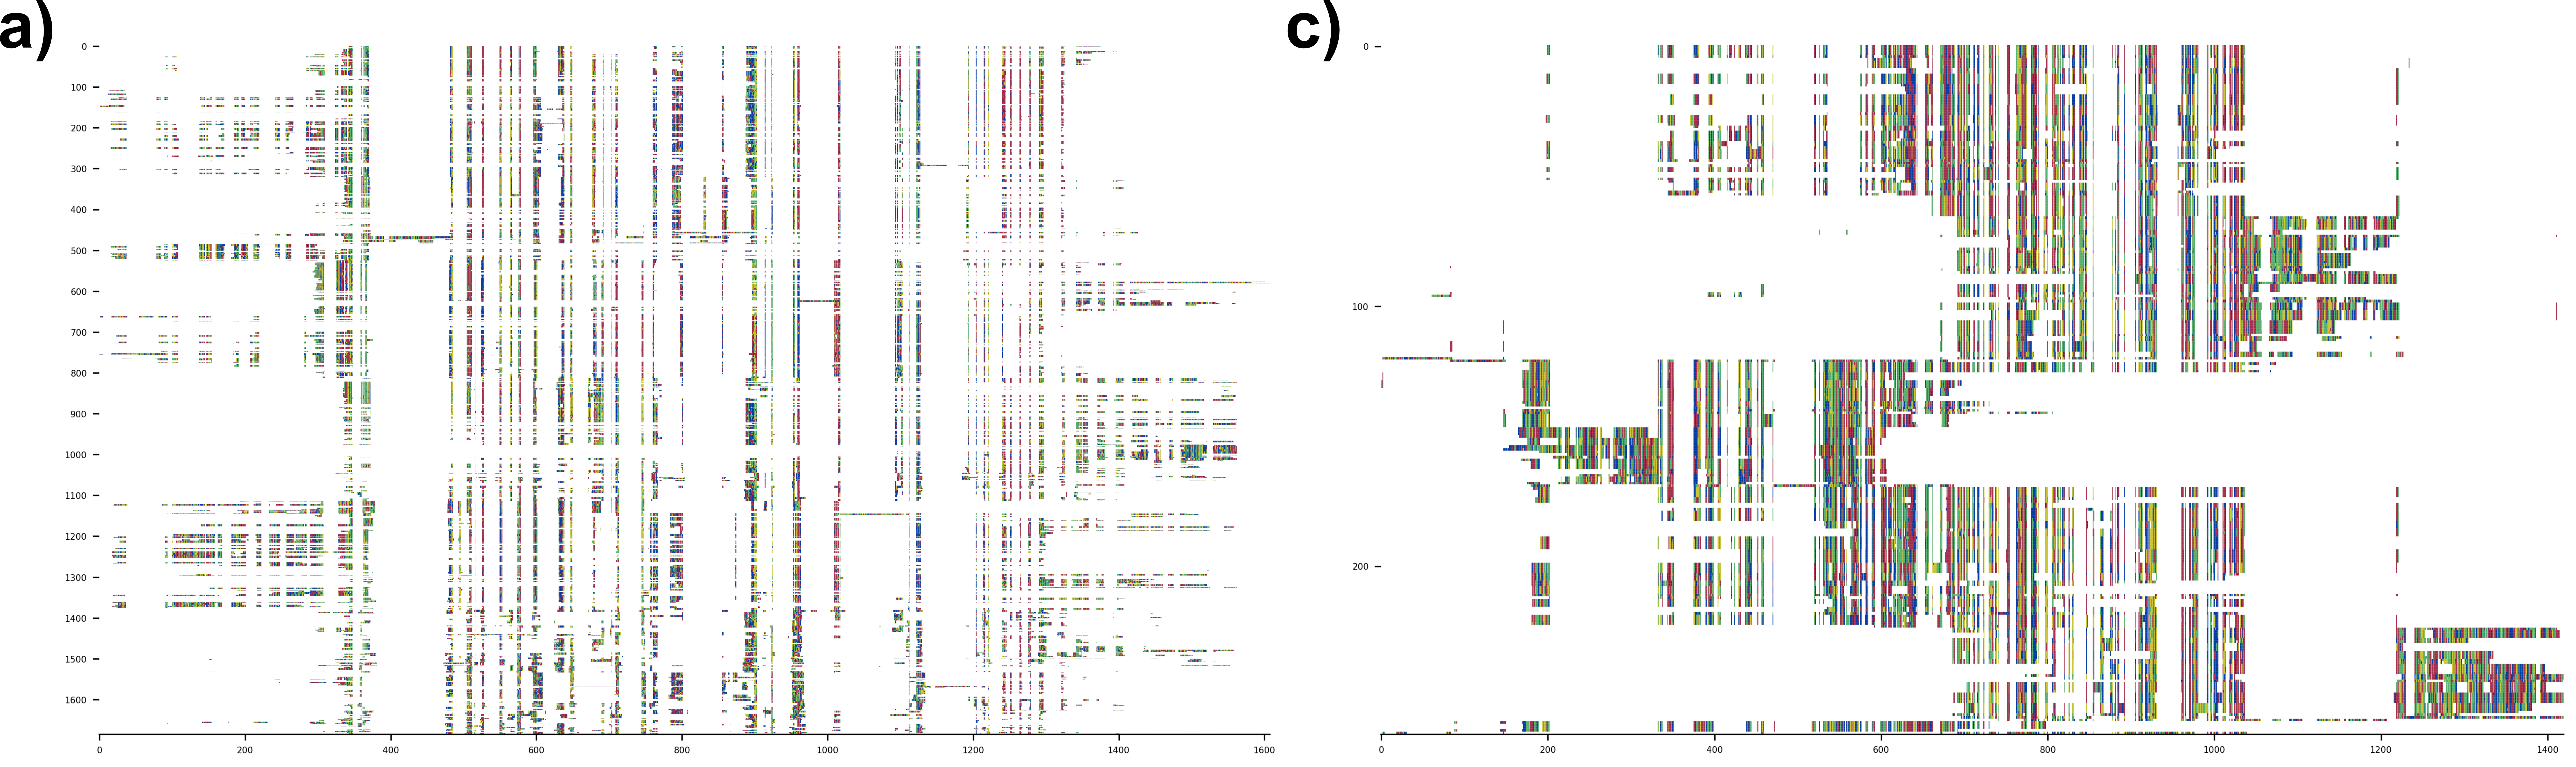
\includegraphics[width=\textwidth]{figs/msas_crypton.png}
    \caption{a) MSA of 1685 sequences of Crypton sequences. Alignment length 1607 bp. b) Alignment of the 265 Crypton sequences, selected by the iterative performance methodology. Alignment length: 1419 bp. Nucleotides and gaps are color coded: Adenine: Green, Cytosine: Blue, Guanine: Yellow, Thymine: Red, Gaps: White. MSAs created with MAFFT with the parameters established in Table \ref{table:tab1}. Image generated with CIAlign.}
    \label{fig:image2}
\end{figure*}

The rationale for creating an iterative performance test stemmed from the inability of pHMMs generated using all selected TE sequences to recover the same sequences, thereby failing a basic validation for a pHMM. Figure \ref{fig:image2} provides an overview of the MSA of the 1,685 Crypton TE sequences obtained from the five selected organisms. Figure \ref{fig:image2} shows that the majority of the MSA is composed of gaps inserted by MAFFT and the chosen local alignment algorithm. The total length of the alignment is 1607 bp. This exceeds the median length of 140 bp of the selected Crypton sequences (Supplementary Data S3 - Figure 10). In regards to the pHMM created using as a basis this MSA, Table 3 shows the statistics obtained from the output of \textit{hmmbuild}. 

\begin{table}[!t]
\caption{Parameters from the Crypton pHMM of 1,685 sequences and 265 sequences. Obtained using the \textit{hmmbuild} tool from the HMMER software suite. The following parameters are defined: \textit{nseqs}: The number of sequences in the provided MSA. \textit{alen}: The effective alignment length. \textit{mlen}: The effective consensus positions of the MSA used by hmmbuild to create the pHMM. \textit{eff\_nseqs}: The number of sequences used to estimate the profile. \textit{re-pos}: The relative entropy per position of the pHMM.} \label{table:tab3}
\begin{tabularx}{\columnwidth}{@{} X l l l l l @{}}
\toprule
\textbf{Name} & \textbf{nseqs} & \textbf{alen} & \textbf{mlen} & \textbf{eff\_nseq} & \textbf{re-pos}\\
\midrule
\textbf{Crypton pHMM} & 1685 & 1607 & 461 & 1685 & 0.487 \\
\textbf{Sel. Crypton pHMM} & 265 & 1419 & 539 & 265 & 0.547 \\
\bottomrule
\end{tabularx}
\end{table}
\raggedbottom

Among the parameters in Table \ref{table:tab3}, \textit{mlen} is particularly informative as it represents the consensus positions from which the pHMM is composed. The \textit{hmmbuild} tool selected only 461 out of 1,607 possible columns as valuable positions to represent the MSA, constituting just 28\% of the total MSA length. Using this pHMM to search for the sequences from which it was constructed yields poor results. It would be expected that the pHMM could detect all the sequences it was created from, but as shown in \textbf{Table 4 A)}, without any filtering, only half of the sequences are detected. Narrowing the results to only the top strand reduces detection to just 12\% of the total sequences. This performance issue is problematic when using pHMMs with TEs and was observed across other analyzed superfamilies (\textbf{Supplementary Data S4} has more information on this).
To query sequences to the pHMM, the nhmmer tool was used. The results provide various levels of information, and it is up to the user to decide where to start. Querying a sequence with nhmmer can generate results where different segments of the same sequence match different parts of the profile and can also generate reverse complements of the queried sequences, expanding the search space. To ensure reliability, only unique hits with an e-value below 0.01 and on the top strand were considered throughout the analysis. The lower the e-value, the more significant the hit. An e-value of 0.01 suggests that, on average, about one false positive would be expected in every 100 searches with different query sequences \cite{sean_r_eddy_hmmer_2023}. 

To improve the base MSA for any given pHMM, we proposed the iterative performance test. As stated in the Materials and Methods section, the chosen measure of quality for selecting an MSA is the number of sequences that the pHMM created from it can recover. The pHMM is created from a training dataset, and its performance is tested on a separate testing dataset. The iterative performance test begins with a pairwise alignment of all the selected sequences. For example, with 1,685 sequences of the Crypton TE, there would be $1,685 x 1,685 = 2,839,225$ alignments. The pairwise scores of the sequences are sorted from largest to smallest. Given a fixed group size (e.g., 5 sequences), it is possible to generate 336 groups ($1680/5$) of training and testing datasets. The last group (1685 in this case) is avoided because it represents the entire dataset of sequences.

Figure \ref{fig:image3} shows the plot of recovered sequences from each of the created pHMMs in the iterative performance test. It was expected that the curve would follow a logistic growth (as indicated by the blue dashed line), but this was not the case. A peak of recovered sequences occurred at 265 sequences, indicating that this MSA produces the pHMM capable of recovering the most sequences from an unknown dataset, making it the best performer. Table \ref{table:tab4} \textbf{B} and \ref{table:tab4} \textbf{C} show the raw number data of the selected 265-sequence pHMM against the test dataset (1,420 sequences) and the complete set of Crypton sequences (1,685 sequences). Comparatively, it is possible to observe an overall increase in the sequences found by the pHMM. Regarding the unique sequences found, both cases show an increment when querying the 265-sequence pHMM against the complete dataset (Table \ref{table:tab4} \textbf{C}). Regarding the parameters of the new pHMM, we can see an improvement on the consensus positions selected by \textit{hmmbuild} when using 265 (Table \ref{table:tab3} (\textbf{Sel. Crypton pHMM})) sequences vs 1685 sequences (Table \ref{table:tab3} (\textbf{Crypton pHHM})) of the Crypton TE. Comparatively speaking, we have 539 consensus positions. That is 78 more positions than the original model (461). This is directly seen in the MSA produced by these 265 sequences (\textbf{Supplemental Data - Figure 11}). In contrast with the original MSA (Figure \ref{fig:image2}) we see a reduction of the gaps and a more cohesive set of columns.

\subsection{Phylogenetic constraints.}\label{subsec3_3}
\begin{figure*}[t]%
    \centering
    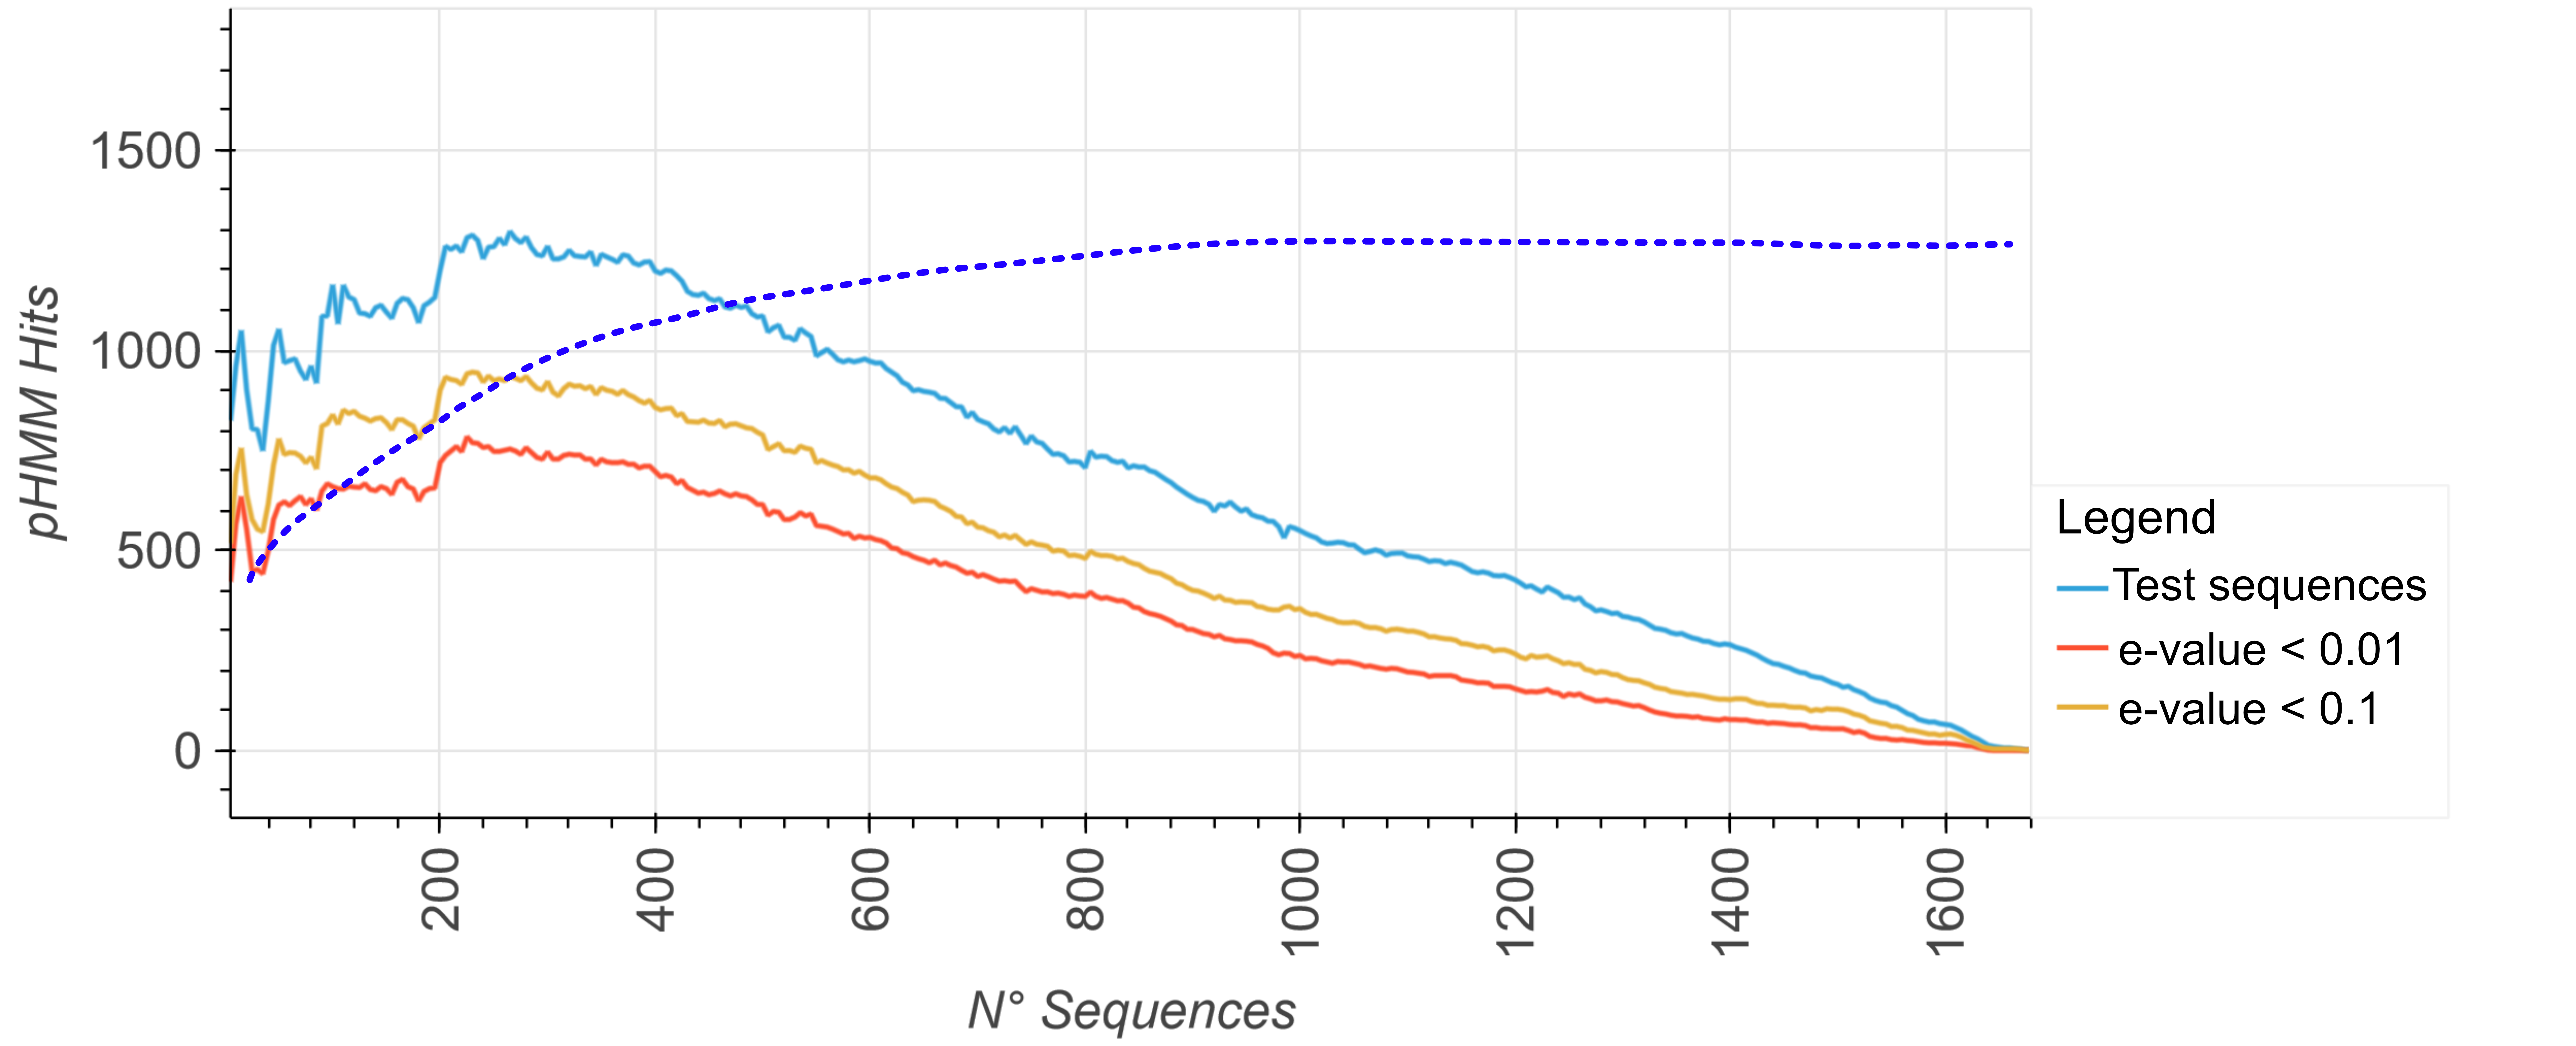
\includegraphics[width=\textwidth]{figs/best_msa_cryp.png}
    \caption{pHMM Hits vs. Recovered Sequences - Crypton TE Superfamily: This plot illustrates the iterative performance test using groups of 5 sequences, added iteratively until the entire dataset is covered. Each point represents the results of the corresponding pHMM against the test dataset. The cyan curve depicts the total recovered sequences, the yellow curve shows the total sequences with an e-value below 0.1, and the red curve represents the total sequences with an e-value below 0.01. The dashed blue line represents the expected behavior of this test.}
    \label{fig:image3}
\end{figure*}
As previously stated, there is a direct link between the results obtained from a pHMM and the sequences of the MSA it is based on. Increasing the specificity of sequence selection results in a higher number of recovered sequences by the pHMM. This leads to a more cohesive MSA in terms of useful consensus positions, allowing tools like \textit{hmmbuild} to infer relationships to other sets of sequences more effectively. Phylogenetic inference ensures the proposed relationships through two main factors: branch length and confidence values at tree nodes. The \textit{Shimodaira–Hasegawa} approximate likelihood ratio test (SH-aLRT) and the ultrafast bootstrap test (UFBoot) are used for this purpose. Bootstrapping is a sampling technique used in phylogenetics to assess the robustness of inferred phylogenetic trees. Traditional bootstrap methods involve generating multiple replicate datasets (from the MSA) through resampling with replacement, rerunning the phylogenetic analysis on each replicate dataset, and then summarizing the results to estimate branch support. SH-aLRT is a statistical test designed to provide more accurate and efficient assessments of branch support compared to standard bootstrap analyses \cite{shimodaira_multiple_1999,guindon_new_2010}. Using the information provided by a phylogenetic tree, we can extract sequence relationships based on fixed thresholds of branch length and confidence. These thresholds can be adjusted to obtain a minimal set of sequences from which a new MSA will be created and used as the basis for the pHMM. A script (phylo\_analysis.py) automates this process and analyzes the 13 superfamilies of TEs. By adjusting the minimum branch length and maximum bootstrap value, we can find the minimum number of sequences in the remaining tree connections.

Applying this methodology, we observe an increase in the sequences recovered by a pHMM in selected cases, along with a reduction in the sequences needed to generate the pHMM itself. This is demonstrated in Table 6, which shows the results for the 5S-Deu-L2 TE superfamily using both the iterative performance test and the phylogenetic constraint methodology. In both cases, a reduction in sequences is observed, reaching a minimum of 22 sequences that can detect 30\% of the test dataset, based on branches with a length less than 0.31. When using a bootstrap value greater than 95, 124 sequences are selected, indicating high confidence in the inferred relationships for the entire tree of 145 sequences. Although an increase in pHMM performance was seen, this was not the case for every tested superfamily.

Supplementary Data S7 contains tables with the results of the phylogenetic restrictions applied to the 13 superfamilies of the analyzed TEs. This allows us to hypothesize that the increase in pHMM performance is directly related to an increment in sequence identity. Both critical steps of the proposed methodology (sequence selection and phylogenetic constraints) aim to achieve this. The impact of these steps on pHMM performance is discussed in the next section.

\subsubsection{Percentage of sequence identity as a crucial factor in performance of TEs.}\label{subsubsec3_1}
\begin{table*}[!t]
\caption{pHMM Results: \textbf{A)} 1,685 sequences of Crypton TE vs. the same queried sequences. \textbf{B)} Selected 265 sequences from the iterative performance test vs. 1,420 sequences of the corresponding test dataset. \textbf{C)} Selected 265 sequences from the iterative performance test vs. 1,685 sequences of Crypton TE. Numbers were extracted from the output file produced by nhmmer. }
\label{table:tab4}
\begin{tabular*}{\textwidth}{@{\extracolsep{\fill}}lcccccc@{\extracolsep{\fill}}}
\toprule
 &
  \multicolumn{1}{l}{\textbf{A) Normal}} &
  \multicolumn{1}{l}{} &
  \multicolumn{1}{l}{\textbf{B) Selected}} &
  \multicolumn{1}{l}{} &
  \multicolumn{1}{l}{\textbf{C) Selected}} &
  \multicolumn{1}{l}{} \\
\textbf{Crypton} &
  \multicolumn{1}{l}{\textbf{pHMM Hits}} &
  \multicolumn{1}{l}{\textbf{Pct.}} &
  \multicolumn{1}{l}{\textbf{pHMM Hits}} &
  \multicolumn{1}{l}{\textbf{Pct.}} &
  \multicolumn{1}{l}{\textbf{pHMM Hits}} &
  \multicolumn{1}{l}{\textbf{Pct.}} \\
\midrule
All                     & 875           & 51.93\%              & 1296          & 91.3\%               & 1761          & 104.5\%              \\
Unique                  & 627           & 37.21\%              & 853           & 60.1\%               & 1103          & 65.5\%               \\
e-value \textless 0.01  & 342           & 20.30\%              & 527           & 37.1\%               & 762           & 45.2\%               \\
Top strand              & 205           & 12.17\%              & 259           & 18.2\%               & 406           & 24.1\%               \\
Comp. strand            & 137           & 8.13\%               & 268           & 18.9\%               & 356           & 21.1\%               \\
\textbf{Total of Seqs.} & \textbf{1685} & \multicolumn{1}{l}{} & \textbf{265}  & \multicolumn{1}{l}{} & \textbf{265}  & \multicolumn{1}{l}{} \\
\textbf{Queried Seqs.}  & \textbf{1685} & \multicolumn{1}{l}{} & \textbf{1420} & \multicolumn{1}{l}{} & \textbf{1685} & \multicolumn{1}{l}{} \\
\bottomrule
\end{tabular*}
\end{table*}
\raggedbottom

Sequence identity, in the context of DNA or proteins, refers to the extent of similarity between two sequences. It is typically expressed as a percentage and represents the proportion of identical residues (nucleotides in DNA or amino acids in proteins) shared between the two sequences when they are aligned. As MSAs form the basis of the methodologies used in this work, sequence identity is a crucial factor to consider. Sequence identity is directly affected by mutations, including insertions, deletions, base changes, and indels (random insertions and deletions). A higher percentage of similarity often indicates a common evolutionary origin or a recent duplication event. As such, sequence identity can vary between different superfamilies of TEs, and different copies of the same TE can vary in identity. As previously stated, this variability is directly related to the poor conservation of TEs in general terms. The high mutation rate leads to greater divergence among copies of TEs, both between genomes and within different superfamilies of TEs in a genome \cite{phimister_mobile_2017, bourque_ten_2018, arkhipova_giant_2019}. To assess the impact of these variations on pHMMs, a series of mutation simulations were performed. Using a developed in-house script and considering a base sequence length, a fixed number of sequences, and a fixed number of changes, we generated as many changes as the length allowed. The base sequence was created by a function that generates random DNA sequences with random nucleotide percentages, and this base sequence was replicated to achieve the selected total number of sequences.

Considering the desired mutation and the number of changes, the function alters all of the sequences in an ordered manner, but with random states for each change applied to each sequence. For example, in a set of 10 sequences of length 100, changes will be applied iteratively, increasing by 10 changes each time until reaching 90 changes. Using deletions as an example, in the first iteration, a set of 10 sequences with no changes is created. In the next iteration, a new set of 10 sequences is created with 10 random deletions in each sequence. This process continues until the last step, where 90 deletions are applied. For insertions, a specific number of insertions are placed at random positions in the sequence. If a position is repeated, it is discarded. For base changes, a random choice among the four nucleotides is made at random positions, with no correction if the new nucleotide is the same as the original. For indels, it is randomly decided whether an insertion or deletion occurs at the chosen positions.
For each set of sequences with mutations, a pHMM is created and used to find the original sequences without any modifications. Figure 5 shows the results of simulations for sequences of length 100 bp in different quantities (100, 400, 1000, and 3000). It is evident that around 60\% sequence identity, the number of sequences recovered by a pHMM starts to rapidly decrease. Base changes have the least impact, maintaining close to 50\% identity before the number of recovered sequences drops. In contrast, deletions have the highest impact, with recovered sequences beginning to fall around 80\% identity, depending on the sequence length.
Figure 6 illustrates the impact of sequence identity on sequences recovered by the pHMMs of TE superfamilies. Figure 6a shows that TEs generally cluster where pHMMs struggle to recover sequences, indicating low average sequence identity. Some families, like MULE-MuDR, deviate from this trend and show higher sequence recovery rates but still do not recover all original sequences (Supplementary Data S4). Figure 6b demonstrates the effect of the iterative performance test, showing that selected sequences from each TE superfamily have higher sequence identity, resulting in better recovery rates by the corresponding pHMMs. Extreme cases like MULE-MuDR, Penelope, and PiggyBac superfamilies exhibit significant increases in sequence identity. The results of applying phylogenetic constraints (branch distance and bootstrap values) are shown in Figures 6c and 6d. Both methods highlight the previously mentioned extreme cases, but branch distance selection has a more pronounced effect on sequence identity and the sequences recovered by the pHMMs.
Overall, the simulations show the importance of sequence identity with respect to the number of sequences that a particular pHMM can recover. The sequence identity TEs is low on average, being detrimental when using pHMM to identify them.

\subsection{pHMM results.}\label{subsec3_4}
Figure 7 shows an overview of the recuperated sequences (hits) per pHMM (a) and the median identity of the used sequences to create those pHMM (b). Overall the base results (in both plots) are lower than any other of the proposed methodologies (blue line). 
The iterative performance methodology shows an improvement in pHMM hits across all analyzed superfamilies except Kolobok (red line). Branch distance selection demonstrates a higher improvement compared to other methodologies, except in the PiggyBac superfamily, where the iterative performance test performs better. Bootstrap selection does not show an improvement, except in the MULE-MuDR superfamily, where it achieves the same result as the branch distance selection. In some extreme cases, such as LTR, branch distance selection shows a drastic improvement over all other selection methodologies.
When considering the median identity of the selected sequences, the iterative performance test does not show an improvement over the base sequences. However, branch distance selection significantly improves the median identity of the sequences. Detailed results of these findings are shown in Supplementary Data S8.
In conclusion, out of the 13 analyzed TE superfamilies, 6 benefit from the iterative performance test (Crypton, I-Jockey, L1-Tx1, Merlin, PiggyBac, tRNA-Deu), 6 benefit from branch distance selection (5s-Deu-L2, DNA, Helitron, LTR, MULE-MuDR, Penelope), and 1 benefits from using the base sequences (Kolobok).

\section{Discussion}\label{sec4}

As a general conclusion, pHMMs face significant challenges in detecting TEs when following a direct path in their creation. This difficulty is evident in the results obtained for the analyzed superfamilies, where no pHMM based on these TEs could completely recover the sequences from which they were created (Supplementary Data S4). Therefore, the proposed methodology serves as an automated refinement of sequence selection to address such cases, aiming to improve the recovery of sequences by any given pHMM. This objective was largely achieved, with only 1 of the 13 analyzed cases (Kolobok) showing a reduction (Supplementary Data S7). As detailed in Figure 7 and Supplementary Data S8, the iterative performance test and branch distance selection methodologies yield the best results for recovering TE sequences with a pHMM. One key factor influencing these results is the sequence identity of the selected sequences. Figure 7 demonstrates that sequence identity increases when using branch distance for selection, which aligns with the concept of sequence similarity as it relates to branch distance in a phylogenetic tree. Although bootstrap values are useful for determining the validity of phylogenetic trees and their branches, they do not aid in improving pHMM results when selecting sequences. Despite analyzing 13 superfamilies, it is not possible to generalize which methodology would work across all known TEs. Consequently, the performance test and phylogenetic constraints must be applied on a case-by-case basis.

Creating MSAs using sequences with a high degree of divergence produces poor results in most MSA tools \cite{hubley_accuracy_2022}. Since this is a common characteristic of TE sequences, poor performance is somewhat expected without manual curation. The detailed methodology proposed in this work serves as an extension to the current usage of pHMMs regarding TEs. DFAM, an open-access database of repetitive DNA elements, represents each family with an MSA and a pHMM. DFAM has used these pHMMs to annotate genomes of various species, with results available for download and use as input for further annotations. As a collaborative effort, DFAM encourages the addition of new information about repetitive elements. With the proposed methodology, it is possible to expand the current selection of available pHMMs in different organisms. In this work, a series of TE pHMMs for different superfamilies of a group of primates (\textit{Callithrix jacchus}, \textit{Gorilla gorilla}, \textit{Homo sapiens}, \textit{Macaca mulatta}, and \textit{Pan paniscus}) were created. These are presented in Table 7 along with the corresponding classification scheme of DFAM. The methodology serves the basic purpose of refining sequence selection and is not limited to any specific organism, provided there is an existing base of TE annotations. In addition to the DFAM classification scheme, each TE has a name corresponding to associated naming conventions in the RepeatMasker information. For example, the Crypton superfamily in humans is composed of \textit{Eulor6A}, \textit{Eulor6B}, \textit{Eulor6C}, \textit{Eulor6D}, \textit{Eulor6E}, \textit{UCON62}, and \textit{MER134} TEs, with the following pHMMs: DF000000132.4, DF000000133.4, DF000000134.4, DF000000135.4, DF000000136.5, DF000001288.2, and DF0000\-00731.5, respectively. A complete list of the DFAM pHMMs used is available in \textbf{Supplementary Data S9.}

Regarding comparisons, the developed pHMMs used the general superfamily category to gather TEs and carry out the aforementioned process. The RepeatMasker annotations for the Human genome were obtained from NCBI Refseq Database, accessed Thu Mar 17 2022. Data from TEs position were extracted using the \textit{bedtools} software (Table 1). DFAM annotations were downloaded from their website for the corresponding pHMMs. DFAM delivers two sets of results, complete and non redundant hits. In this case the complete dataset of hits is being used.


\section{Conclusion}\label{sec5}

TE annotation is a cumbersome process \cite{ou_benchmarking_2019, branco_overview_2023}. Automatic discovery and annotation tools can facilitate and streamline this process, making it accessible to a broader audience dealing with genomic data. Adding tools that enhance the detection process can help mitigate some of the uncertainties that often arise from automation tools. In the proposed methodology, sequence identity is fundamental for selecting base sequences when generating a pHMM. This preselection reduces the size of the initial sequence set, enabling phylogenetic analysis with tools like IQ-TREE. Phylogenetic analysis and the creation of associated phylogenetic trees are essential for applying branch distance selection. This process improves the sequences used to create the pHMM compared to also analyzed bootstrap values. However, this preselection may exclude important information, such as fragmented TE sequences. This, along with the different species, could partially explain discrepancies with analyzed DFAM profiles. Although fragmented TE sequences interfere with creating a more cohesive pHMM, which hinders the detection of sequences, these discrepancies highlight the differences between annotation methodologies. It was expected to have a common base between DFAM and RepeatMasker, especially when analyzing the human genome. This raises questions about the viability of sequence annotation methods in complex scenarios like TEs. The proposed methodology is applicable and could be expanded to a broader selection of organisms. By aligning more closely with DFAM and comparing annotation results, we can consider expanding the database with pHMM profiles that are not readily available.

\section{Data Availability}
The developed scripts, (msa\_calculations.py, phylo\_analysis.py and plotting.py) along with the simulated and used data of this work is available at \url{https://github.com/kako-f/pHMM_TEs}. Supplemental material is available through … and a compressed file in the root of the repository webpage.

\section{Competing interests}
No competing interest is declared.

\section{Author contributions statement}

Must include all authors, identified by initials, for example:
S.R. and D.A. conceived the experiment(s),  S.R. conducted the experiment(s), S.R. and D.A. analysed the results.  S.R. and D.A. wrote and reviewed the manuscript.

\section{Acknowledgments}
The authors thank the anonymous reviewers for their valuable suggestions. This work is supported in part by funds from the National Science Foundation (NSF: \# 1636933 and \# 1920920).


\bibliographystyle{plain}
\bibliography{thesis.bib}

%USE THE BELOW OPTIONS IN CASE YOU NEED AUTHOR YEAR FORMAT.
%\bibliographystyle{abbrvnat}
%\bibliography{reference}


%% sample for biography with author's image
\begin{biography}{{\color{black!20}\rule{77pt}{77pt}}}{\author{Author Name.} This is sample author biography text. The values provided in the optional argument are meant for sample purposes. There is no need to include the width and height of an image in the optional argument for live articles. This is sample author biography text this is sample author biography text this is sample author biography text this is sample author biography text this is sample author biography text this is sample author biography text this is sample author biography text this is sample author biography text.}
\end{biography}

%% sample for biography without author's image
\begin{biography}{}{\author{Author Name.} This is sample author biography text this is sample author biography text this is sample author biography text this is sample author biography text this is sample author biography text this is sample author biography text this is sample author biography text this is sample author biography text.}
\end{biography}

\end{document}
